% -*- root: ../thesis.tex -*-
%!TEX root = ../thesis.tex
% ******************************* Thesis Chapter 5 ****************************


% ----------------------- paths to graphics ------------------------

% change according to folder and file names
\graphicspath{{5/figures/}}

The larger question following the work on P\'olya-Gamma variables and other augmentation works such as \citet{nguyenRobustStudentSt2012} or \citet{henaoBayesianNonlinearSupport2014} is:
What likelihoods have a scale mixture representation?

% and can a general rule be inferred?
This article, extending the work of \citet{palmer2006variational} partially answers by finding a class of functions, the positive-definite radial functions, guaranteed to be interpretable as scale mixtures of Gaussians.
The paper also provides an algorithm to directly infer the \ac{CAVI} updates and Gibbs sampling algorithm from the likelihood.

\textbf{\underline{Authors:}}\\
Th\'eo Galy-Fajou,$^{1}$, Florian Wenzel,$^{2}$, Manfred Opper$^1$\\
\small{$^1$TU Berlin, Germany, $^2$Google Research\\

\textbf{\underline{Details:}}\\
Type: Conference article
Submitted: October 2019\\
Accepted: December 2019\\
URL: \url{https://proceedings.mlr.press/v108/galy-fajou20a.html}\\
Conference: AISTATS 2020\\
License: \href{Creative Commons Attribution (CC BY 4.0)}{https://creativecommons.org/licenses/by/4.0/}\\
% ----------------------- contents from here ------------------------
\newpage
\underline{\textbf{Contributions:}}\\
For an explanation of the terms see the \href{https://mdpi-res.com/data/contributor-role-instruction.pdf}{Contributor Roles Taxonomy} (CReditT)\\
\begin{center}
\begin{tabular}{c|c|c|c|}
    & T.G-F. & F.W. & M.O.\\\hline
    \textbf{Conceptualization} & \checkmark & \checkmark & \checkmark\\
    \textbf{Methodology} & \checkmark & & \\
    \textbf{Formal Analysis} & \checkmark & \checkmark & \checkmark\\
    \textbf{Software} & \checkmark & & \\
    \textbf{Investigation} & \checkmark & & \\
    \textbf{Writing - Original Draft} & \checkmark & \checkmark &\\
    \textbf{Writing - Review \& Editing} & \checkmark & \checkmark & \checkmark\\
    \textbf{Supervision} & & & \checkmark\\
    \textbf{Funding Acquisition} & & & \checkmark
\end{tabular}
\end{center}

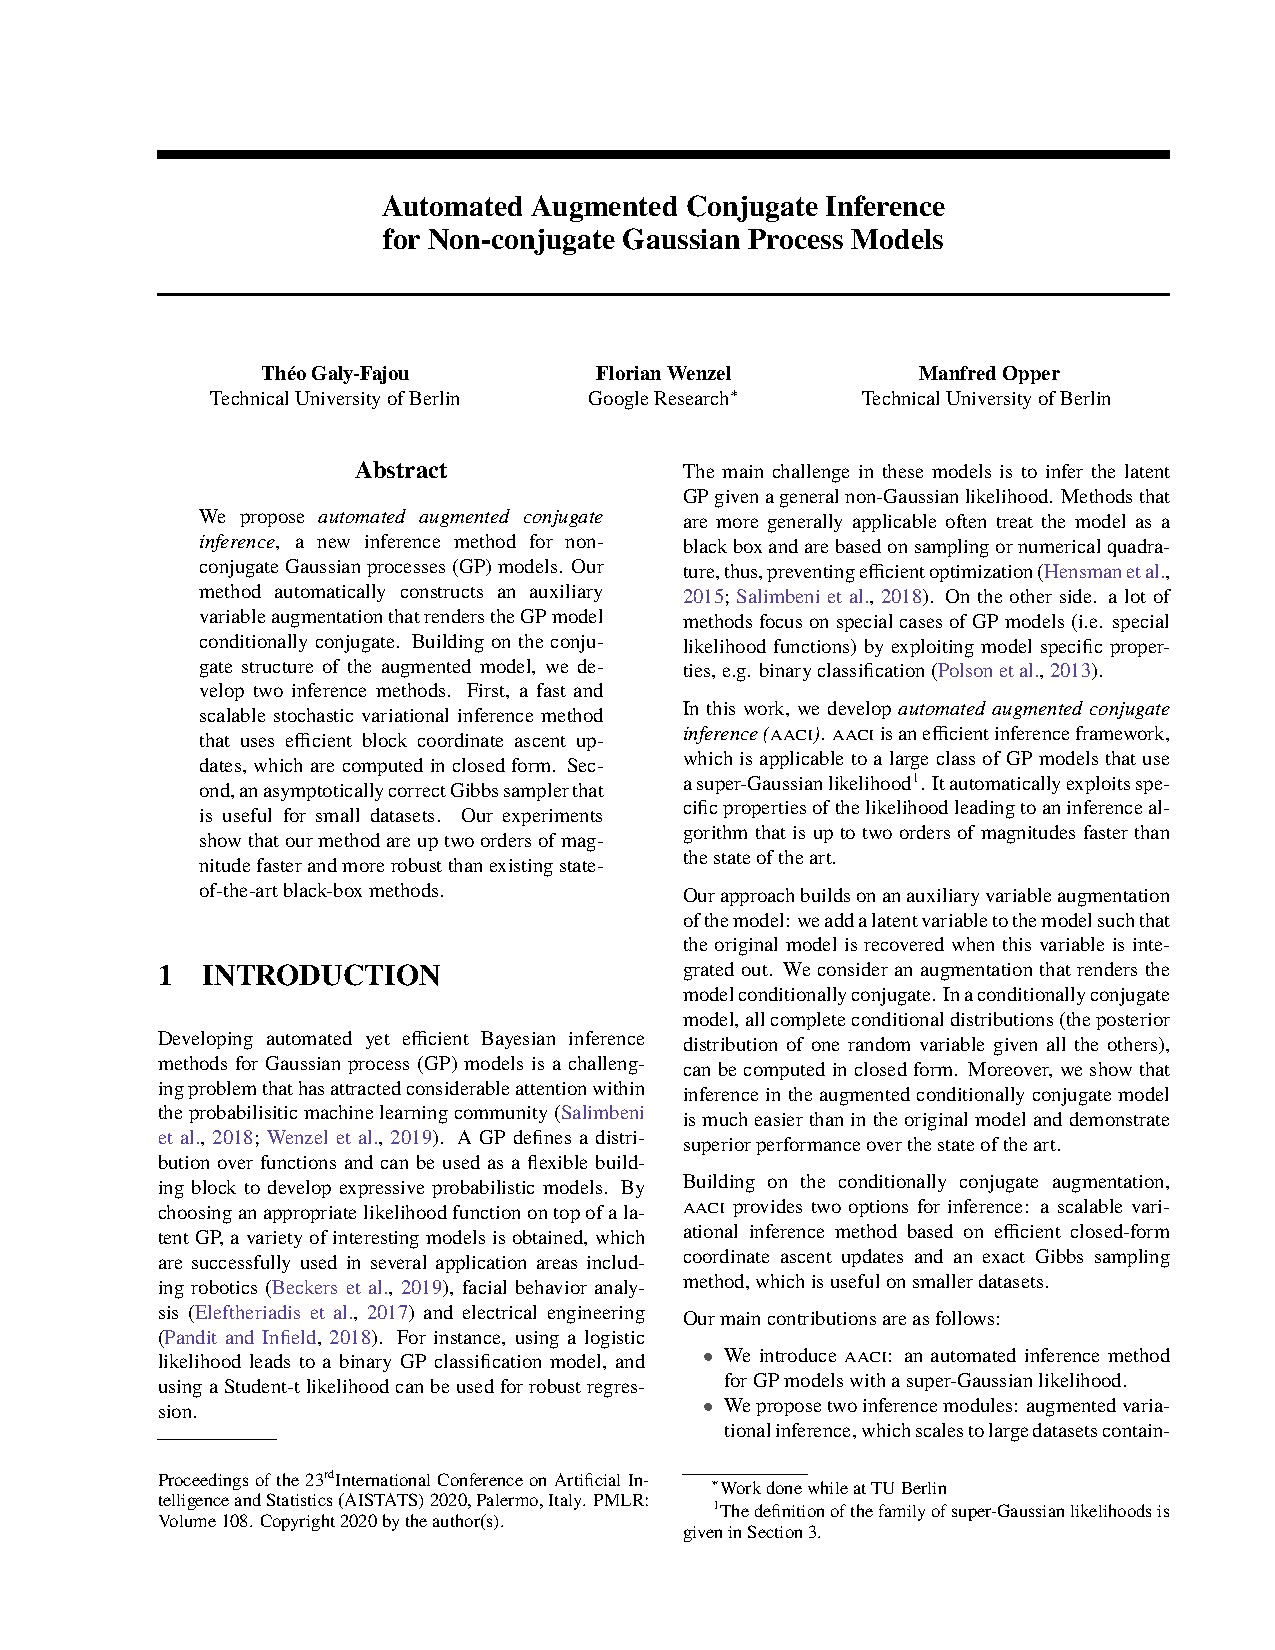
\includepdf[pages=-,pagecommand={},scale=0.95]{./papers/galy-fajou20a.pdf}
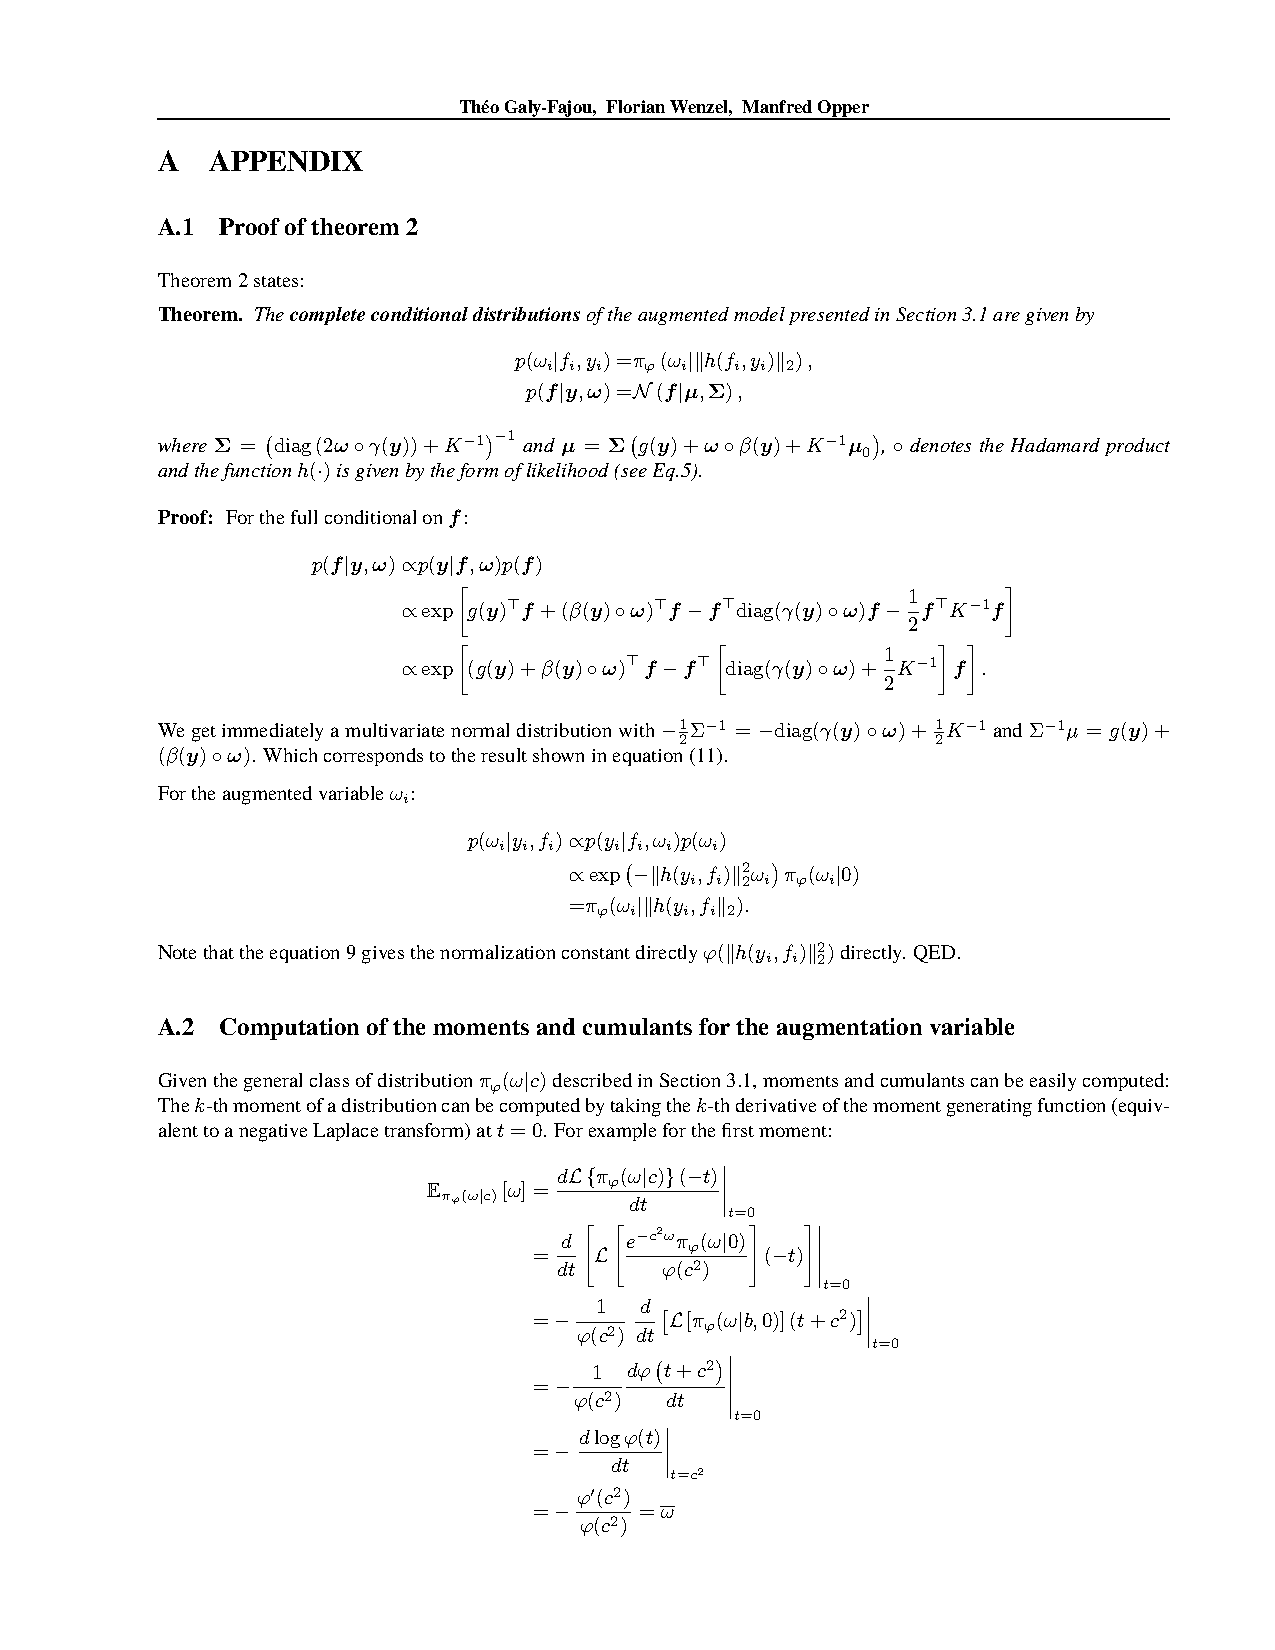
\includepdf[pages=-,pagecommand={},scale=0.95]{./papers/galy-fajou20a-supp.pdf}

% ---------------------------------------------------------------------------
%: ----------------------- end of thesis sub-document ------------------------
% ---------------------------------------------------------------------------

